\section{Despliegue local}\label{sec:impl_local}
Para arrancar el desarrollo del proyecto, se implementa una versión local del
sistema, que permita trabajar en un entorno controlado y sin dependencias
externas para comprobar su correcto funcionamiento y establecer
las configuración base para su posterior despliegue en la nube.

Puesto que se ha decidido utilizar Docker para la gestión de contenedores, se
crea un archivo \texttt{docker-compose.yml} que define los servicios
necesarios para el proyecto, es decir, \textit{Kafka}, \textit{Zookeeper},
\textit{Elasticsearch}, \textit{Kibana} y \textit{Logstash}, ignorando por
el momento la ingesta de datos y la escalabilidad del sistema.

Para la configuración de los servicios, se ha creado un archivo \texttt{.env}
que define las variables de entorno necesarias para el correcto funcionamiento
de los servicios, como las contraseñas o la versión del \textit{stack}.

Esta sección de la documentación documenta el desarrollo de la historia de
usuario inicial, de acuerdo con lo establecido en la sección \fullref{sec:planif_inicial}:

\begin{table}[H]
	\centering
	\begin{tabular}{|p{0.7\linewidth}|c|c|}
		\hline
		\textbf{Nombre} & \textbf{Prioridad} & \textbf{Tamaño} \\
		\hline
		\hline
		Creación de la infraestructura base (técnica) & P0\cellcolor{red!50} & L\cellcolor{orange!50} \\
		\hline
  	\end{tabular}
  	\caption{Lista de HUs cumplimentadas con el despliegue local}
  	\label{tab:impl_local}
\end{table}


\newpage{}
\subsection{Explicación del código}
\emph{El código de despliegue local se encuentra en \fullref{anexo:local}.}

A nivel de configuración, se definen variables de entorno para cada contenedor
mediante el uso de la palabra clave \texttt{environment} y las claves definidas
por cada imagen. Para cada contenedor, se define además información adicional
dependiendo de las características del servicio, como la dependencia en otras
imágenes, los límites de recursos o los puertos de escucha.

Para evitar el ruido excesivo por consola una vez arrancado los servicios, se
reduce el nivel de \textit{logging} a \textit{WARN} en los servicios que lo
soporten.

Durante el arranque de los contenedores, se ejecuta un script de inicialización
que se encarga de crear las credenciales y los usuarios necesarios para el
funcionamiento de los servicios. Estas credenciales son necesarias ya que los
contenedores funcionan mediante tráfico HTTPS.

Los contenedores cuentan con comprobaciones de salud (o \textit{health-checks})
básicas para asegurar que los servicios se han arrancado correctamente y están
funcionando.

Al comienzo del archivo \texttt{docker-compose.yml}, se definen los volúmenes y
las redes necesarias para el correcto funcionamiento de los servicios.

\begin{lstlisting}[style=yaml, caption={Definición de volúmenes y redes en Docker Compose}]
volumes:
	es01data:
	kibanadata:
	elasticdata:
	logstashdata:
	kafkadata:
	certs:

networks:
	default:
		driver: bridge
\end{lstlisting}

A continuación, se definen los servicios necesarios para el proyecto, comenzando
por el contenedor de preparación de credenciales y usuarios. Se utiliza una
imagen de Elasticsearch para la creación de las credenciales, y se monta un
volumen para la persistencia de las mismas.

\begin{lstlisting}[style=yaml, caption={Definición del servicio de preparación}]
setup:
	image: docker.elastic.co/elasticsearch/elasticsearch:${STACK_VERSION}
	volumes:
		- certs:/usr/share/elasticsearch/config/certs
	user: root
	container_name: setup
	command: >
		bash -c '
			if [ x${ELASTIC_PASSWORD} == x ]; then
			echo "Set the ELASTIC_PASSWORD environment variable in the .env file";
			exit 1;
			elif [ x${KIBANA_PASSWORD} == x ]; then
			echo "Set the KIBANA_PASSWORD environment variable in the .env file";
			exit 1;
			fi;
			if [ ! -f config/certs/ca.zip ]; then
			echo "Creating CA";
			bin/elasticsearch-certutil ca --silent --pem -out config/certs/ca.zip;
			unzip config/certs/ca.zip -d config/certs;
			fi;
			if [ ! -f config/certs/certs.zip ]; then
			echo "Creating certs";
			echo -ne \
			"instances:\n"\
			"  - name: es01\n"\
			"    dns:\n"\
			"      - es01\n"\
			"      - localhost\n"\
			"    ip:\n"\
			"      - 127.0.0.1\n"\
			"  - name: kibana\n"\
			"    dns:\n"\
			"      - kibana\n"\
			"      - localhost\n"\
			"    ip:\n"\
			"      - 127.0.0.1\n"\
			> config/certs/instances.yml;
			bin/elasticsearch-certutil cert --silent --pem -out config/certs/certs.zip --in config/certs/instances.yml --ca-cert config/certs/ca/ca.crt --ca-key config/certs/ca/ca.key;
			unzip config/certs/certs.zip -d config/certs;
			fi;
			echo "Setting file permissions"
			chown -R root:root config/certs;
			find . -type d -exec chmod 750 \{\} \;;
			find . -type f -exec chmod 640 \{\} \;;
			echo "Waiting for Elasticsearch availability";
			until curl -s --cacert config/certs/ca/ca.crt https://es01:9200 | grep -q "missing authentication credentials"; do sleep 1; done;
			echo "Setting kibana_system password";
			until curl -s -X POST --cacert config/certs/ca/ca.crt -u "elastic:${ELASTIC_PASSWORD}" -H "Content-Type: application/json" https://es01:9200/_security/user/kibana_system/_password -d "{\"password\":\"${KIBANA_PASSWORD}\"}" | grep -q "^{}"; do sleep 10; done;
			echo "All done!";
		''

	healthcheck:
		test: [ "CMD-SHELL", "[ -f config/certs/es01/es01.crt ]" ]
		interval: 5s
		timeout: 10s
		retries: 10
\end{lstlisting}

El servicio de preparación necesita tener una comprobación de salud, puesto que
el resto de contenedores lo tienen marcado como dependencia para su arranque. En
este caso, la comprobación consiste en la existencia de un archivo de
certificado.

Una vez definido el servicio de preparación, se definen los servicios de
\textit{Kafka} y \textit{Zookeeper}, que se basan en imágenes oficiales de
\textit{Confluent}.

\begin{lstlisting}[style=yaml, caption={Definición de los servicios de Kafka}]
zookeeper:
	container_name: zookeeper
	image: confluentinc/cp-zookeeper:latest
	environment:
	ZOOKEEPER_CLIENT_PORT: 2181
	ZOOKEEPER_TICK_TIME: 2000
	ZOO_LOG4J_PROP: WARN,CONSOLE
	ports:
	- 2181:2181

kafka:
	container_name: kafka
	image: confluentinc/cp-kafka:latest
	depends_on:
		- zookeeper
		- es01
	ports:
		- 9092:9092
		- 29092:29092
	environment:
		KAFKA_BROKER_ID: 1
		KAFKA_ZOOKEEPER_CONNECT: zookeeper:2181
		KAFKA_ADVERTISED_LISTENERS: LISTENER_DOCKER_INTERNAL://kafka:29092,LISTENER_DOCKER_EXTERNAL://localhost:9092
		KAFKA_LISTENER_SECURITY_PROTOCOL_MAP: LISTENER_DOCKER_INTERNAL:PLAINTEXT,LISTENER_DOCKER_EXTERNAL:PLAINTEXT
		KAFKA_INTER_BROKER_LISTENER_NAME: LISTENER_DOCKER_INTERNAL
		KAFKA_OFFSETS_TOPIC_REPLICATION_FACTOR: 1
		KAFKA_LOG4J_ROOT_LOGLEVEL: WARN
		KAFKA_TOOLS_LOG4J_LOGLEVEL: ERROR
		KAFKA_LOG4J_LOGGERS: 'kafka=WARN,kafka.controller=WARN,kafka.log.LogCleaner=WARN,state.change.logger=WARN,kafka.producer.async.DefaultEventHandler=WARN'
\end{lstlisting}

Ambos servicios cuentan con una serie de variables de entorno que definen su
configuración, como el puerto de escucha, el \textit{broker ID} o la dirección
de \textit{Zookeeper}.

Una vez definidos los servicios de Kafka, se define el servicio más crítico, el
contenedor de Elasticsearch, del que depende el funcionamiento de todo el
sistema.

\begin{lstlisting}[style=yaml, caption={Definición del servicio de Elasticsearch}]
es01:
    image: docker.elastic.co/elasticsearch/elasticsearch:${STACK_VERSION}
    container_name: es01
    restart: unless-stopped
    depends_on:
      - setup
    environment:
      - node.name=es01
      - cluster.name=${CLUSTER_NAME}
      - discovery.type=single-node
      - bootstrap.memory_lock=true
      - logger.level=WARN
      - ELASTIC_PASSWORD=${ELASTIC_PASSWORD}
      - xpack.security.enabled=true
      - xpack.security.http.ssl.enabled=true
      - xpack.security.http.ssl.key=certs/es01/es01.key
      - xpack.security.http.ssl.certificate=certs/es01/es01.crt
      - xpack.security.http.ssl.certificate_authorities=certs/ca/ca.crt
      - xpack.security.transport.ssl.enabled=true
      - xpack.security.transport.ssl.key=certs/es01/es01.key
      - xpack.security.transport.ssl.certificate=certs/es01/es01.crt
      - xpack.security.transport.ssl.certificate_authorities=certs/ca/ca.crt
      - xpack.security.transport.ssl.verification_mode=certificate
    ulimits:
      memlock:
        soft: -1
        hard: -1
      nofile:
        soft: 65536
        hard: 65536
    cap_add:
      - IPC_LOCK
    labels:
      co.elastic.logs/module: elasticsearch
      co.elastic.metrics/module: elasticsearch
    volumes:
      - es01data:/usr/share/elasticsearch/data
      - certs:/usr/share/elasticsearch/config/certs
    ports:
      - 9200:9200
    healthcheck:
      test:
        [
          "CMD-SHELL",
          "curl -s --cacert config/certs/ca/ca.crt https://localhost:9200 | grep -q 'missing authentication credentials'"
        ]
      interval: 10s
      timeout: 10s
      retries: 10
\end{lstlisting}

Debido a que se trata del servicio más importante y grande, se requieren muchas
opciones de configuración, como la limitación de recursos, la persistencia de
datos o la configuración de seguridad. Como en el resto de servicios, se define
una comprobación de salud que se encarga de comprobar que el servicio está
disponible.

Para simplificar lo máximo posible la arquitectura de este prototipo, tan solo
se define un nodo de Elasticsearch, aunque la configuración de escalabilidad
sería sencilla gracias al diseño de Docker.

Por último, se definen los servicios de Kibana y Logstash, que dependen de
Elastic.

\begin{lstlisting}[style=yaml, caption={Definición de los servicios de Kibana}]
kibana:
    container_name: kibana
    image: docker.elastic.co/kibana/kibana:${STACK_VERSION}
    restart: unless-stopped
    volumes:
      - kibanadata:/usr/share/kibana/data
      - certs:/usr/share/kibana/config/certs
    environment:
      SERVER_NAME: kibana
      SERVER_PORT: 5601
      SERVER_HOST: 0.0.0.0
      ELASTICSEARCH_HOSTS: https://es01:9200
      ELASTICSEARCH_USERNAME: kibana_system
      ELASTICSEARCH_PASSWORD: ${KIBANA_PASSWORD}
      ELASTICSEARCH_SSL_CERTIFICATEAUTHORITIES: config/certs/ca/ca.crt
      LOGGING_ROOT_LEVEL: warn
      XPACK_ENCRYPTEDSAVEDOBJECTS_ENCRYPTIONKEY: ${KEY}
      XPACK_REPORTING_ENCRYPTIONKEY: ${KEY}
      XPACK_SECURITY_ENCRYPTIONKEY: ${KEY}
    links:
      - es01
    depends_on:
      - setup
      - es01
    labels:
      co.elastic.logs/module: kibana
      co.elastic.metrics/module: kibana
    ports:
      - 5601:5601
    healthcheck:
      test:
        [
          "CMD-SHELL",
          "curl -s -I http://localhost:5601 | grep -q 'HTTP/1.1 302 Found'"
        ]
      interval: 10s
      timeout: 10s
      retries: 10
\end{lstlisting}

\begin{lstlisting}[style=yaml, caption={Definición de los servicios de Logstash}]
logstash:
    container_name: logstash
    image: docker.elastic.co/logstash/logstash:${STACK_VERSION}
    restart: unless-stopped
    user: root
    volumes:
      - logstashdata:/usr/share/logstash/data
      - certs:/usr/share/logstash/certs
    environment:
      - ELASTIC_HOSTS="https://es01:9200"
      - ELASTIC_USER="elastic"
      - ELASTIC_PASSWORD=${ELASTIC_PASSWORD}
      - log.level=warn
      - xpack.monitoring.enabled=false
    command: >
      bash -c "echo 'input { kafka { bootstrap_servers => \"kafka:29092\" topics => [\"laravel-logs\"] } } output { elasticsearch { hosts => [\"https://es01:9200\"] user => \"elastic\" password => \"${ELASTIC_PASSWORD}\" ssl => true cacert => \"certs/ca/ca.crt\" } }' > /usr/share/logstash/pipeline/logstash.conf; bin/logstash -f /usr/share/logstash/pipeline/logstash.conf"
    ports:
      - 5000:5000
    depends_on:
      - es01
      - kafka
      - setup
    labels:
      co.elastic.logs/module: logstash
      co.elastic.metrics/module: logstash
    links:
      - es01
      - kibana
\end{lstlisting}

Se hace uso de la red interna de Docker para facilitar la comunicación entre los
contenedores, y se definen comprobaciones de salud para asegurar que los
servicios se han arrancado correctamente. Para Logstash, se define un script de
lanzamiento que genera el archivo de configuración y ejecuta el servicio, aunque
podría montarse un volumen con el archivo de configuración ya generado.

\newpage{}
\subsection{Uso del sistema}
Una vez arrancados los contenedores mediante el comando
\texttt{docker compose up}, se puede acceder a los servicios a través de la
dirección local \texttt{localhost}. En el caso de Kibana, se puede acceder a
la interfaz de usuario mediante la dirección \texttt{localhost:5601}. En el
caso de Elasticsearch, se pueden hacer peticiones HTTPS a través de la dirección
\texttt{localhost:9200}. Para Kafka, Zookeeper y Logstash, se pueden hacer
peticiones a través de las direcciones \texttt{localhost:9092},
\texttt{localhost:2181} y \texttt{localhost:9600}, respectivamente.

\begin{figure}[H]
	\centering
	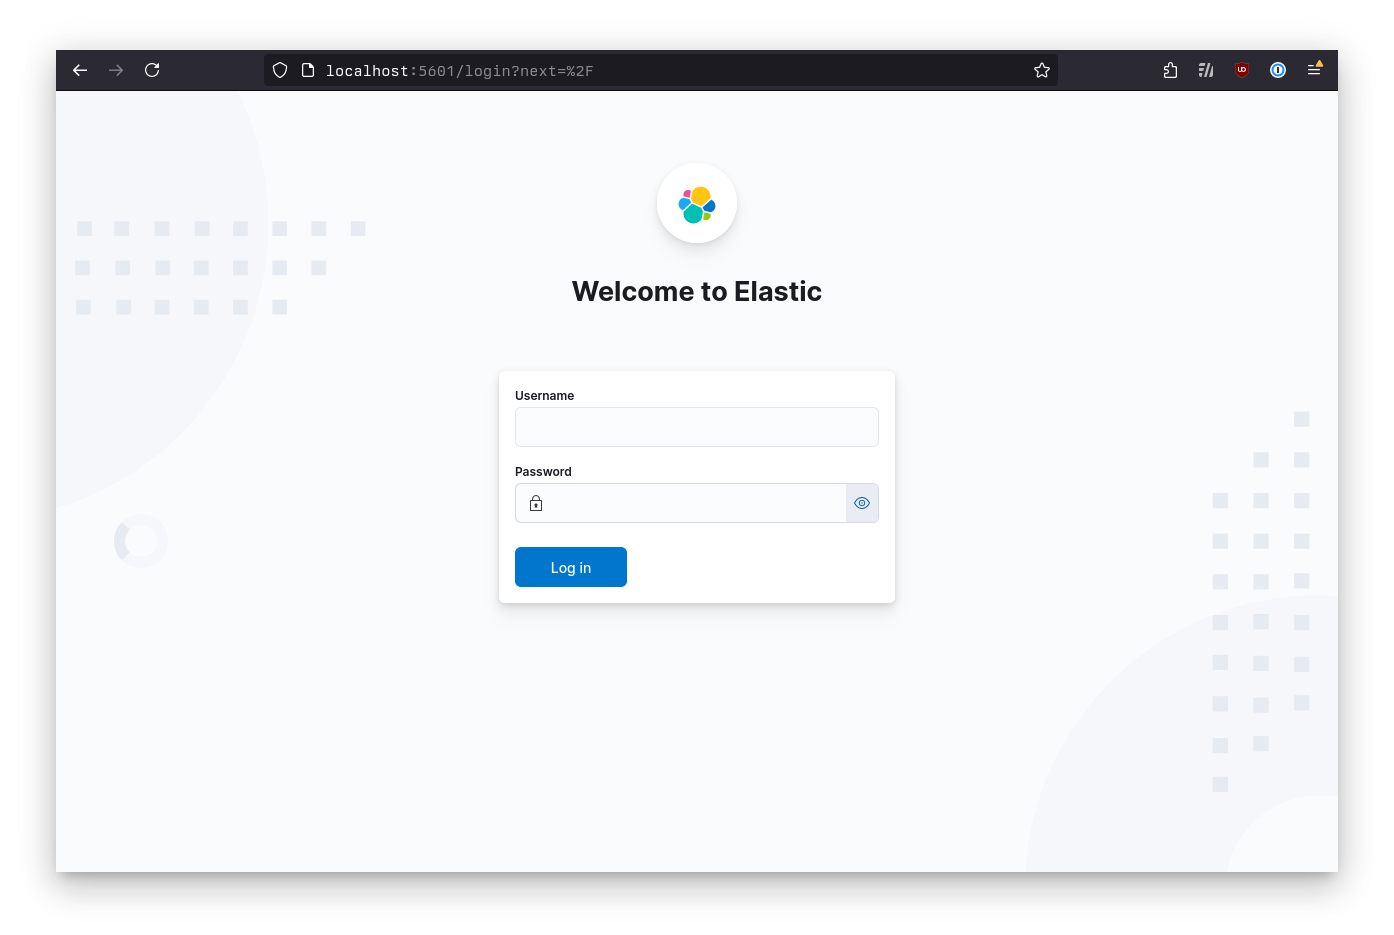
\includegraphics[width=\textwidth]{impl/local1.png}
	\caption{Inicio de sesión en Kibana}
	\label{fig:kibana_login}
\end{figure}

Una vez en la pantalla de inicio de sesión, se puede acceder con las credenciales
definidas en el archivo \texttt{.env} para el usuario \texttt{elastic}.

\begin{figure}[H]
	\centering
	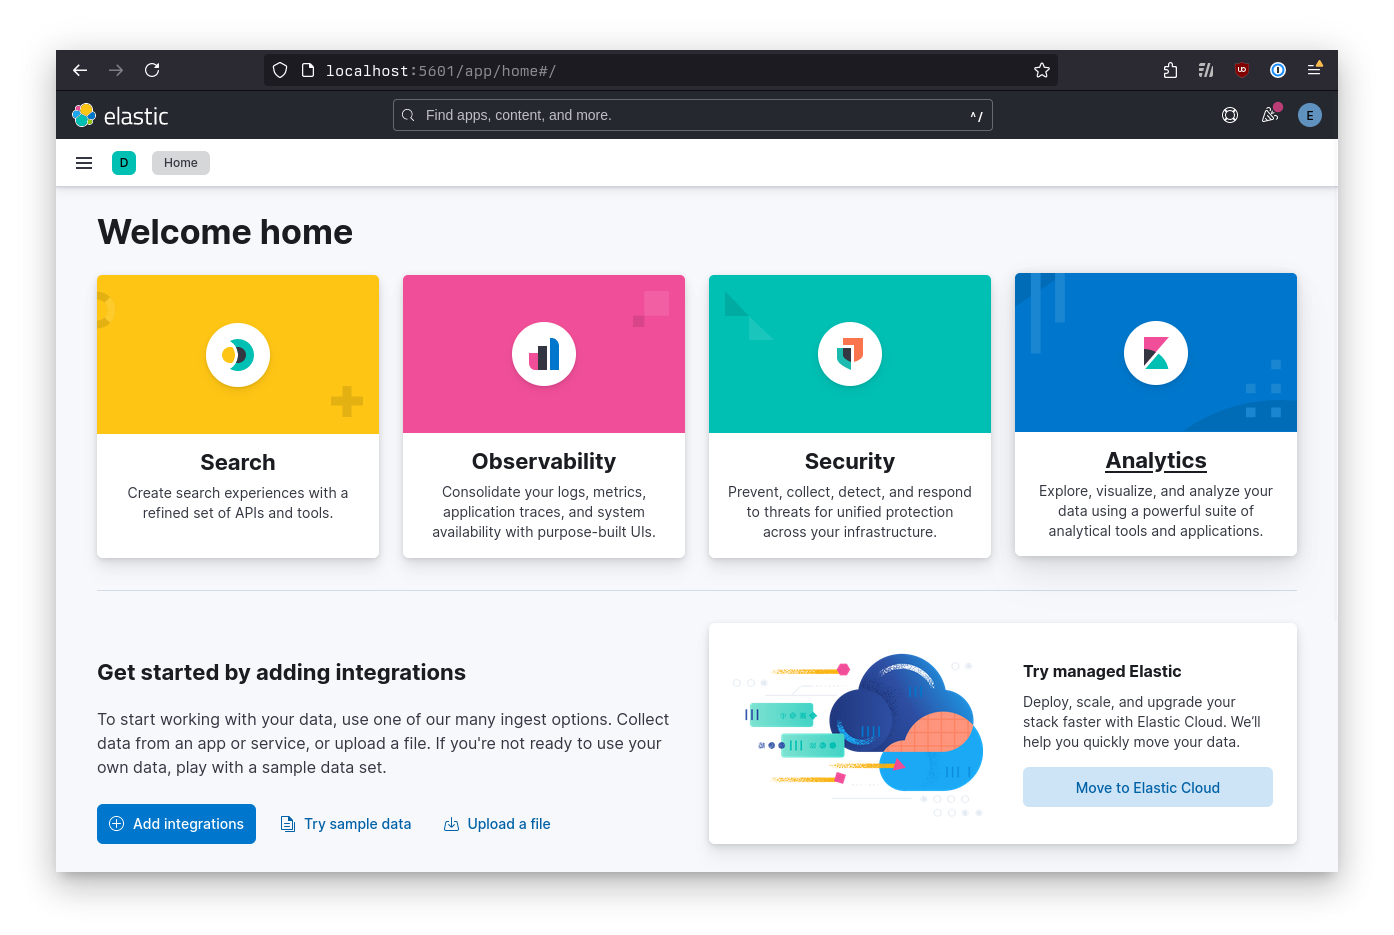
\includegraphics[width=\textwidth]{impl/local2.png}
	\caption{Página de inicio de Kibana}
	\label{fig:kibana_start}
\end{figure}

Una vez aquí, se puede hacer click en la opción \texttt{Try sample data} para
cargar un conjunto de datos de ejemplo y probar la funcionalidad de Kibana con
Elasticsearch. Por supuesto, también se pueden probar la ingesta de datos a
través de Logstash y Kafka o, si así se desea, a través de los \textit{Beats}
especializados de ingesta directa de Elastic.

El manual de uso del sistema se encuentra en \fullref{sec:manual_usuario}.


\newpage{}
\subsection{Proceso de desarrollo}\label{subsec:impl_local_desarrollo}
Para el desarrollo del sistema, se ha seguido un proceso iterativo, comenzando
a partir del ejemplo oficial de Elastic para \textit{Docker Compose}\footnote{
  \url{https://www.elastic.co/blog/getting-started-with-the-elastic-stack-and-docker-compose}
}. A partir de este ejemplo, se añaden progresivamente configuraciones y
servicios, y se prueban las funcionalidades de cada uno de ellos, actualizando
con regularidad el código en el repositorio privado establecido.

\begin{figure}[H]
  \centering
  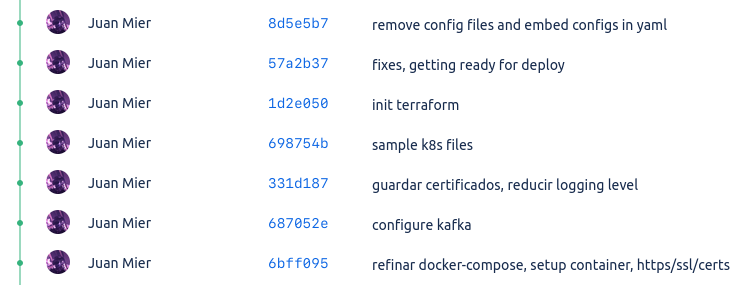
\includegraphics[width=\textwidth]{impl/commits.png}
  \caption{Ejemplo de commits en el repositorio privado}
  \label{fig:commits}
\end{figure}

Inicialmente, se prueban los servicios mínimos (Kibana y Elasticsearch) sin
HTTPS para comprobar su correcto funcionamiento. Una vez se ha comprobado que
los servicios funcionan correctamente, se añade la configuración de seguridad
y se prueban los servicios con HTTPS, ajustando más configuraciones como el
nivel de registro de logs o las comprobaciones de salud de los contenedores.

Una vez se ha comprobado que los servicios funcionan correctamente, se añaden
los servicios de Kafka, Zookeeper y Logstash, y se prueban las conexiones entre
los servicios, ajustando las configuraciones necesarias para que los servicios
se comuniquen correctamente.
